%----------------------------------------------------------------------------------------
%	PACKAGES AND OTHER DOCUMENT CONFIGURATIONS
%----------------------------------------------------------------------------------------

\documentclass[a0,portrait]{a0poster}

\usepackage{multicol}
\columnsep=100pt
\columnseprule=3pt

\usepackage[svgnames]{xcolor}
\definecolor{tudLogoColor}{HTML}{0A4D6C}

%\usepackage{times}
\usepackage{palatino}

\usepackage{graphicx}
\graphicspath{{figures/}}
\usepackage{booktabs}
\usepackage[font=small,labelfont=bf]{caption}
\usepackage{amsfonts, amsmath, amsthm, amssymb}
\usepackage{wrapfig}
\usepackage{multirow}
\usepackage{times}
\usepackage{latexsym}
\usepackage{algorithm}
\usepackage{algpseudocode}
\usepackage[english]{babel}
\usepackage{caption}
\usepackage[caption=false]{subfig}
\usepackage{lipsum}

\begin{document}

%----------------------------------------------------------------------------------------
%	POSTER HEADER 
%----------------------------------------------------------------------------------------
\begin{minipage}[c]{0.25\linewidth}

\includegraphics[width=16.5cm]{logo.png}\\
\end{minipage}
\begin{minipage}[c]{0.75\linewidth}
\veryHuge \color{tudLogoColor} \textbf{Multi-Element Long Distance Dependencies:}\\ % Title
\Huge\textbf{Using SP\emph{k} Languages to Explore the Characteristics of Long Distance Dependencies} \color{Black}\\[1cm] % Subtitle
\huge\fontfamily{put}\textbf{Abhijit Mahalunkar \& Prof. John D. Kelleher}\\[0.5cm]
\huge Technological University Dublin, Ireland\\[0.4cm]
\Large \texttt{abhijit.mahalunkar@mydit.ie \& john.d.kelleher@dit.ie}\\
\end{minipage}

% \vspace{1cm}

%----------------------------------------------------------------------------------------

\begin{multicols}{2}
\fontfamily{pvh}\selectfont

%----------------------------------------------------------------------------------------
%	ABSTRACT
%----------------------------------------------------------------------------------------

%\begin{abstract}
%
%In order to successfully model Long Distance Dependencies (LDDs) it is necessary to understand the full-range of the characteristics of the LDDs exhibited in a target dataset. In this paper, we use Strictly \emph{k}-Piecewise languages to generate datasets with various properties. We then compute the characteristics of the LDDs in these datasets using mutual information and analyze the impact of factors such as (i) \emph{k}, (ii) length of LDDs, (iii) vocabulary size, (iv) forbidden subsequences, and (v) dataset size. This analysis reveal that the number of interacting elements in a dependency is an important characteristic of LDDs. This leads us to the challenge of modelling multi-element long-distance dependencies. Our results suggest that attention mechanisms in neural networks may aide in modeling datasets with multi-element long-distance dependencies. However, we conclude that there is a need to develop more efficient attention mechanisms to address this issue.
%
%\end{abstract}

%----------------------------------------------------------------------------------------
%	INTRODUCTION
%----------------------------------------------------------------------------------------

\color{tudLogoColor}

\section*{Introduction}

\color{black}
LDDs are related to the rate of decay of statistical dependence of two points with increasing time interval or spatial distance between them. To date, most research on LDDs has focused on the distance the dependency spans within the sequence. We show the complexity of LDDs not only arises from the distance but also a number of other factors, including: (i) the number of unique symbols in a dataset, (ii) the size of the dataset, (iii) the number of interacting symbols within an LDD, and (iv) the distance between the interacting symbols. We use SP\emph{k} languages to explore the complexity of LDDs.

One aspect of LDDs that has been neglected in the research on LDDs is the complexity that arises from a multi-element dependency (i.e., dependencies that involves interactions between more than 2 elements). By controlling \emph{k} in the SP\emph{k} grammar, it is possible to generate datasets with varying degrees of multi-element dependency. We explore whether attention mechanism can help with multi-element LDDs using two models, Transformer-XL and AWD-LSTM.

%----------------------------------------------------------------------------------------
%	OBJECTIVES
%----------------------------------------------------------------------------------------

\color{tudLogoColor}

\section*{Main Objectives}

\color{black}
\begin{enumerate}
\item Use Strictly \emph{k}-Piecewise languages to generate datasets with varying (i) \emph{k}, (ii) length of LDDs, (iii) vocabulary size, (iv) forbidden subsequences, and (v) dataset size.
\item Compute the characteristics of the LDDs in these datasets using mutual information and analyze the impact of factors.
\item Multi-element dependency can be introduced by varying \emph{k}. 
\item Study how attention mechanisms in neural networks may aide in modeling datasets with multi-element long-distance dependencies.
\end{enumerate}

%----------------------------------------------------------------------------------------
%	METHODS
%----------------------------------------------------------------------------------------

\section*{Methods}

\subsection*{Long Distance Dependency Characteristics}

Mutual information $I(X,Y)$ measures dependence between random variables $X$ and $Y$. These random variables have marginal distributions $p(x)$ and $p(y)$ and are jointly distributed as $p(x,y)$. It can also be expressed using the \emph{entropy} of $X$ and $Y$ i.e. $H(X)$, $H(Y)$ and their \emph{joint entropy}, $H(X,Y)$. The \emph{LDD characteristics} is the function of $I(X,Y)$ w.r.t $D$.

\begin{multicols}{2}
\begin{equation*}
\begin{aligned}
I(X;Y) = H(X) + H(Y) - H(X,Y)
\label{eq:mut-inf-h}
\end{aligned}
\end{equation*}
\begin{equation*}
H(X) = \log N - 1/N \sum_{i=1}^{k} N_i \psi(N_i)
\label{eq:entropy-adj}
\end{equation*}
\\
$D=$ distance between 2 symbols \\
$dataset=$ sequence of letters \\
$|dataset|=$ length of the sequence \\
$N_i=$ frequency of unique symbol \emph{i} \\
$N = \sum N_i$ \\
$K=$ number of unique symbols \\
$\psi(N_i)=$ \emph{logarithmic derivative of the gamma function} of $N_i$ \\

% \begin{itemize}
% \item $D=$ distance between 2 symbols
% \item $dataset[n_1:n_2]=$ sequence between index $n_1$ to $n_2$
% \item $|dataset|=$ length of the sequence
% \item $N_i=$ frequency of unique symbol \emph{i}
% \item $N = \sum N_i$
% \item $K=$ number of unique symbols
% \item $\psi(N_i)=$ \emph{logarithmic derivative of the gamma function} of $N_i$
% \end{itemize}
\columnbreak
\begin{algorithm}[H]
\begin{algorithmic}
 \For{$D\gets 1, |dataset|$}
  \State $X \gets dataset[0:|dataset|-D]$
  \State $Y \gets dataset[D:|dataset|]$
  \State $XY \gets$ zero-matrix of size ($K^X,K^Y$)
  \For{$i\gets 0,|X|$}
    \State Increment $XY[X[i],Y[i]]$
  \EndFor
  \State Compute $N_i^X$, $N^X$, $K^X$ for $X$
  \State Compute $N_i^Y$, $N^Y$, $K^Y$ for $Y$
  \State Compute $N_i^{XY}$, $N^{XY}$, $K^{XY}$ for $XY$
  \State Compute $H(X)$, $H(Y)$ and $H(X,Y)$ %Eq.~\ref{eq:entropy-adj}
  \State $I[D]\gets H(X)+H(Y)-H(X,Y)$
 \EndFor
\caption{LDD Characteristics}\label{ldd_algo}
\end{algorithmic}
\end{algorithm}
\end{multicols}

\subsection*{Strictly \emph{k}-Piecewise}

SP\emph{k} languages form a subclass of regular languages. SP\emph{k} languages are defined by grammar \emph{G}\textsubscript{\emph{SPk}} as a set of permissible \emph{k}-\emph{subsequences}. Here, \emph{k} indicates the number of elements in a dependency. Subsequences which are not in the grammar are called \emph{forbidden subsequences}.

\begin{itemize}
\item \( \Sigma \) = \{\emph{a, b, c, d}\} 
\item \emph{u} = [\emph{bbcbdd}], \emph{v} = [\emph{bbdbbbcbddaa}] and \emph{w} = [\emph{bbabbbcbdd}], where \( \vert \)\emph{u}\( \vert \) = 6, \( \vert \)\emph{v}\( \vert \) = 12 and \( \vert \)\emph{w}\( \vert \) = 10.
\end{itemize}
Strings \emph{u} and \emph{v} are valid SP\emph{2} strings because they are composed of subsequences that are in \emph{G\textsubscript{SP\emph{2}}}. However, \emph{w} is an invalid SP\emph{2} string because \emph{w} contains \{\emph{ab}\} a subsequence which is a \emph{forbidden subsequence}. These constraints apply for any string \emph{x} where \( \vert \)\emph{x}\( \vert \in \mathbb{Z} \).

Let \emph{G\textsubscript{SP\emph{3}}}  = \{\emph{aaa, aab, abb, baa, bab, bba, bbb, ...}\} and \emph{forbidden subsequence} = \{\emph{aba}\} be an SP\emph{3} grammar which is comprised of permissible $3$-\emph{subsequences}. Thus, \emph{u} = [\emph{aaaaaaab}], where \( \vert \)\emph{u}\( \vert \) = 8 is a valid SP\emph{3} string and \emph{v} = [\emph{aaaaabaab}], where \( \vert \)\emph{v}\( \vert \) = 9 is an invalid SP\emph{3} string as defined by the grammar \emph{G\textsubscript{SP\emph{3}}}.

\begin{wrapfigure}{r}{0.2\textwidth}
\begin{center}
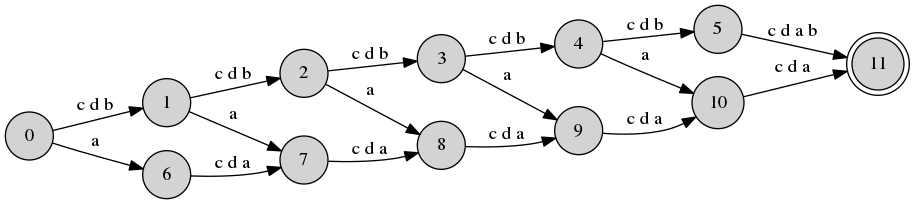
\includegraphics[width=0.2\textwidth]{fsa1.png}
\captionof{figure}{Finite-state diagram of \emph{G\textsubscript{SP2}}}
\label{fig:fsa1}
\end{center}
\end{wrapfigure}

Finite-state diagram of \emph{G\textsubscript{SP2}} is in figure~\ref{fig:fsa1}. The \emph{forbidden subsequence} for this grammar is \{\emph{ab}\}, hence the state diagram has no path that generates strings with \{\emph{ab}\} as a subsequence, \emph{e.g.} \{\emph{abcccc}\}.

%----------------------------------------------------------------------------------------
%	RESULTS 
%----------------------------------------------------------------------------------------

\section*{Results}

\subsection*{LDD Characteristics of datasets}

\begin{center}
\begin{minipage}[b]{0.45\linewidth}
\centering
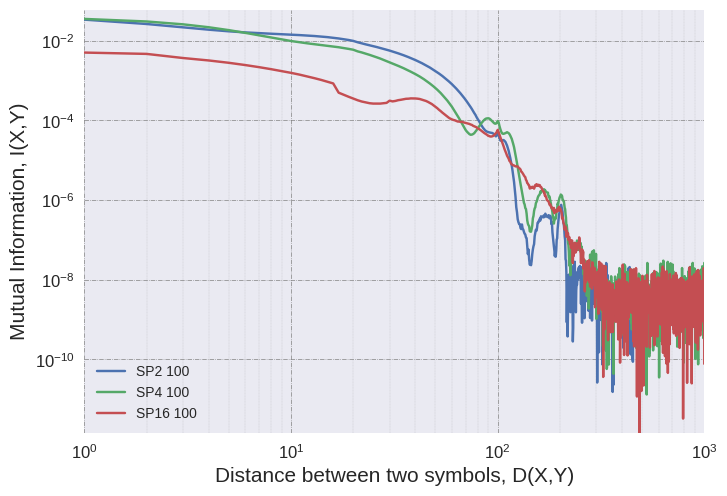
\includegraphics[width=\textwidth]{spk_k.png}
\captionof{figure}{Multi-Element Dependency (\emph{k})}
\label{fig:spk_k}
\end{minipage}
\hspace{0.5cm}
\begin{minipage}[b]{0.45\linewidth}
\centering
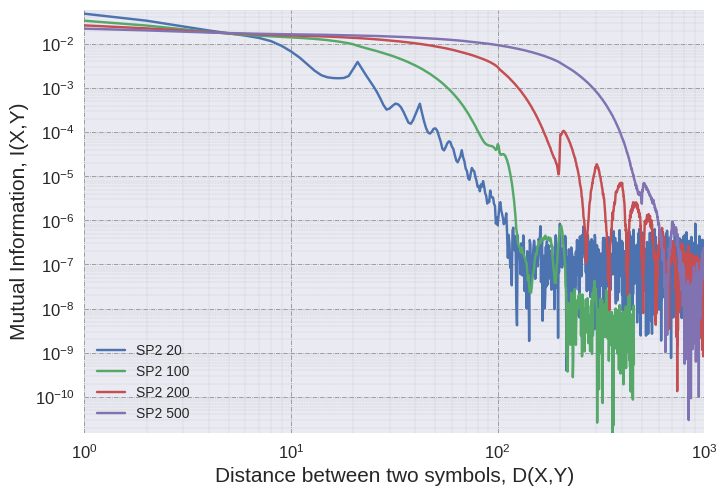
\includegraphics[width=\textwidth]{spk_len.png}
\captionof{figure}{Influence of LDD length}
\label{fig:spk_len}
\end{minipage}
\end{center}

\begin{center}
\begin{minipage}[b]{0.45\linewidth}
\centering
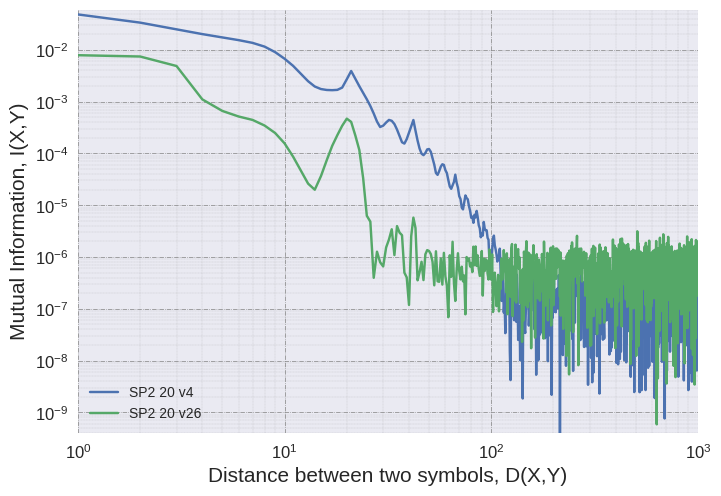
\includegraphics[width=\textwidth]{spk_v.png}
\captionof{figure}{Influence of Vocabulary}
\label{fig:spk_v}
\end{minipage}
\hspace{0.5cm}
\begin{minipage}[b]{0.45\linewidth}
\centering
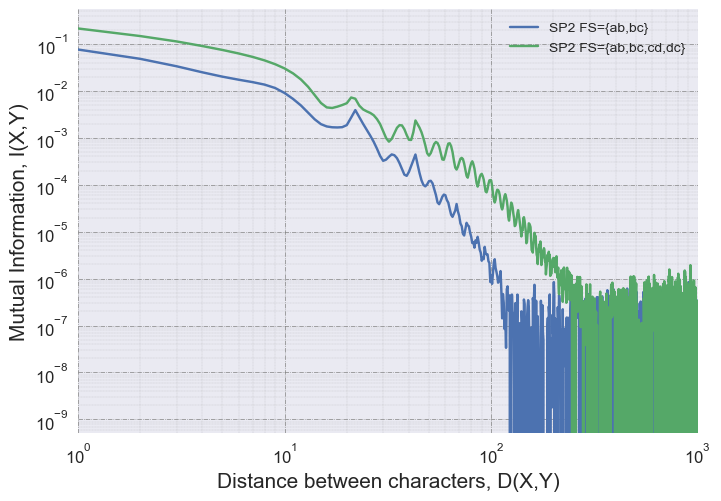
\includegraphics[width=\textwidth]{spk_f.png}
\captionof{figure}{Different \emph{forbidden strings}}
\label{fig:spk_f}
\end{minipage}
\end{center}

\begin{center}
\begin{minipage}[b]{0.45\linewidth}
\centering
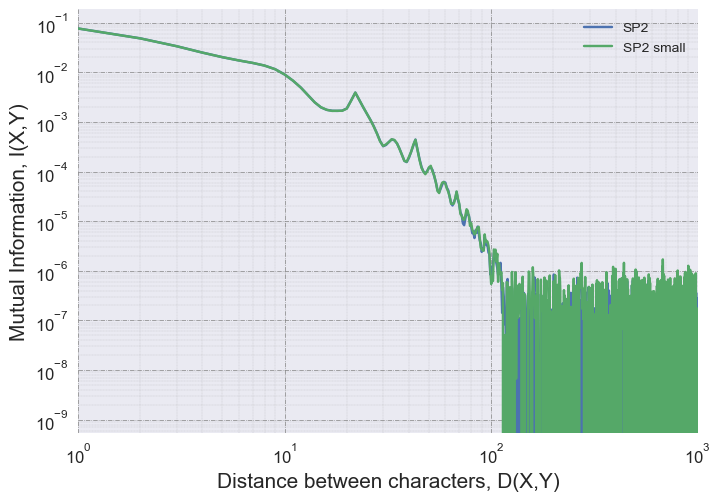
\includegraphics[width=\textwidth]{spk_size.png}
\captionof{figure}{Multi-Element Dependency (\emph{k})}
\label{fig:spk_size}
\end{minipage}
\hspace{0.5cm}
\begin{minipage}[b]{0.45\linewidth}
\centering
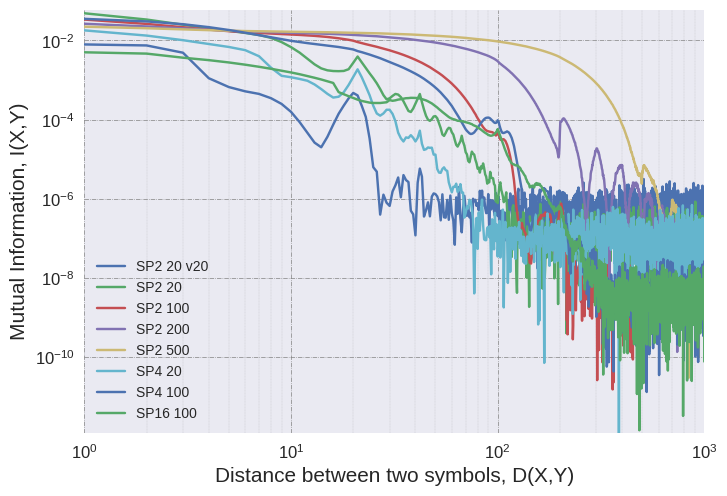
\includegraphics[width=\textwidth]{spk_full.png}
\captionof{figure}{All the datasets}
\label{fig:spk_full}
\end{minipage}
\end{center}

In hac habitasse platea dictumst. Etiam placerat, risus ac.

Adipiscing lectus in magna blandit:

\subsection*{Perplexity of language models}

\begin{center}
\begin{tabular}{c c c c c | c c c c}
\toprule
\multirow{3}{*}{Models} & \multicolumn{8}{c}{Test Perplexity in \emph{bpc}} \\ \cline{2-9}
	& \multicolumn{4}{c|}{Vocabulary size $V{=}4$} & \multicolumn{4}{c}{Vocabulary size $V{=}26$} \\ \cline{2-9}
    & SP$2$ & SP$4$ & SP$8$ & SP$16$ & SP$2$ & SP$4$ & SP$6$ & SP$8$ \\
\midrule
$1$   & $1.6855$ & $1.8038$ & $1.9611$ & $2.0759$ & $4.6846$ & $4.7320$ & $4.7384$ & $4.7385$ \\
$2$   & $1.413$ & $1.486$ & $1.658$ & $1.708$ & $4.525$ & $4.635$ & $4.707$ & $4.708$ \\
\bottomrule
\end{tabular}
\captionof{table}{Perplexity score of $1$: Transformer-XL and $2$: AWD-LSTM models.}
\label{tab:perplexity_score_v4}
\end{center}

\begin{wrapfigure}{r}{0.25\textwidth}
\begin{center}
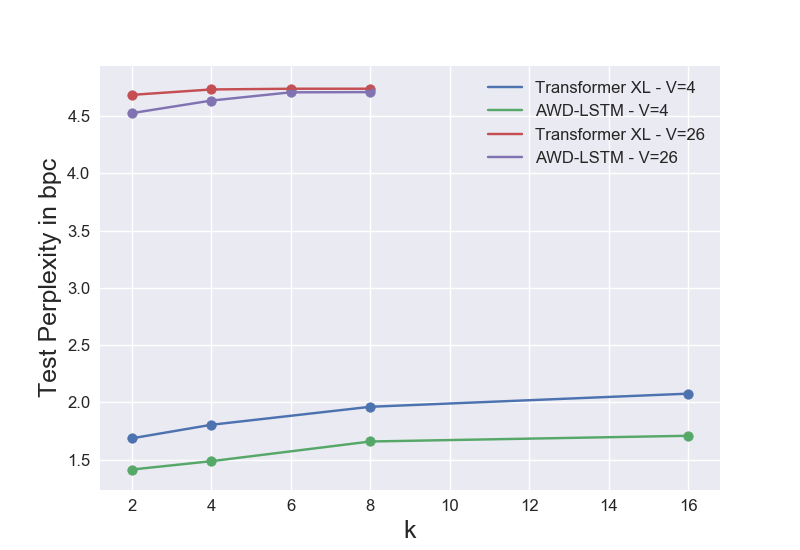
\includegraphics[width=0.25\textwidth]{perplexity.png}
\captionof{figure}{Complex system plots of homogenous sampled datasets}
\label{fig:perplexity}
\end{center}\vspace{1cm}
\end{wrapfigure}

Vivamus sed nibh ac metus tristique tristique a vitae ante. Sed lobortis mi ut arcu fringilla et adipiscing ligula rutrum. Aenean turpis velit, placerat eget tincidunt nec, ornare in nisl. In placerat.

Vivamus sed nibh ac metus tristique tristique a vitae ante. Sed lobortis mi ut arcu fringilla et adipiscing ligula rutrum. Aenean turpis velit, placerat eget tincidunt nec, ornare in nisl. In placerat.

Vivamus sed nibh ac metus tristique tristique a vitae ante. Sed lobortis mi ut arcu fringilla et adipiscing ligula rutrum. Aenean turpis velit, placerat eget tincidunt nec, ornare in nisl. In placerat.

%----------------------------------------------------------------------------------------
%	CONCLUSIONS
%----------------------------------------------------------------------------------------

\section*{Conclusions}

\begin{itemize}
\item The dependencies that occur in sequential data can also be multi-element. Furthermore, the vocabulary size, and the forbidden subsequences within a grammar also contribute to the difficulty of modelling the dependencies within a dataset.
\item Using SP\emph{k} languages it is possible to synthesize sequential datasets and control the complexity of dependencies exhibited in these datasets and using mutual information it's possible to analyze their LDD characteristics.
\item Results suggest that attention mechanisms in neural networks may aide in modeling datasets with multi-element long-distance dependencies. Although we encourage developing more efficient models.
\end{itemize}

%----------------------------------------------------------------------------------------
%	REFERENCES
%----------------------------------------------------------------------------------------

% \nocite{*} % Print all references regardless of whether they were cited in the poster or not
% \bibliographystyle{plain} % Plain referencing style
% \bibliography{sample} % Use the example bibliography file sample.bib

%----------------------------------------------------------------------------------------
%	ACKNOWLEDGEMENTS
%----------------------------------------------------------------------------------------

\section*{Acknowledgements}

This research was partly supported by the ADAPT Research Centre, funded under the SFI Research Centres Programme (Grant 13/RC/2106) and is co-funded under the European Regional Development Funds. The research was also supported by an IBM Shared University Research Award. We gratefully acknowledge the support of NVIDIA Corporation with the donation of the Titan Xp GPU under NVIDIA GPU Grant used for this research.

%----------------------------------------------------------------------------------------

\end{multicols}
\end{document}